% !TEX program = xelatex
\documentclass[aspectratio=169]{beamer}
\usepackage{amsmath}
\usepackage{amssymb}
\usepackage{graphicx}
\usepackage{tcolorbox}
\usepackage{booktabs}
\usepackage{colortbl}
\usepackage{xcolor}
\usepackage{tikz}
\usetikzlibrary{angles,quotes}
\usepackage[utf8]{inputenc}

% Custom colors
\definecolor{primary}{RGB}{41, 128, 185}
\definecolor{secondary}{RGB}{52, 152, 219}
\definecolor{accent}{RGB}{231, 76, 60}
\definecolor{lightgray}{RGB}{236, 240, 241}

% Theme customization
\usetheme{Madrid}
\usecolortheme{whale}
\setbeamercolor{structure}{fg=primary}
\setbeamercolor{background canvas}{bg=white}
\setbeamercolor{normal text}{fg=black}

% Title page info
\title{Pre-Calculus 11}
\subtitle{Chapter 3.8: Trigonometry Summary / 三角函數總結}
\author{Created by Yi-Chen Lin}
\date{\today}

\begin{document}

% Title Page
\begin{frame}
    \titlepage
\end{frame}

% Overview
\begin{frame}{Chapter 3.8 Overview / 本章總覽}
    \begin{tcolorbox}[colback=lightgray,colframe=primary,title=Topics Covered]
        \footnotesize
        \begin{itemize}
            \item 3.1 Basic Trigonometric Functions
            \item 3.2 Angles in Standard Position
            \item 3.3 Special Triangles
            \item 3.4 Solving Angles in All Four Quadrants
            \item 3.5 Sine Law
            \item 3.6 Ambiguous Case of the Sine Law
            \item 3.7 Cosine Law
        \end{itemize}
    \end{tcolorbox}
\end{frame}

% 3.1 Basic Trigonometric Functions
\begin{frame}{3.1 Basic Trigonometric Functions / 基本三角函數}
    \begin{tcolorbox}[colback=lightgray,colframe=primary,title=Key Points]
        \footnotesize
        \begin{itemize}
            \item Sine, Cosine, Tangent: $\sin\theta$, $\cos\theta$, $\tan\theta$
            \item SOH-CAH-TOA: $\sin\theta = \frac{\text{Opp}}{\text{Hyp}}$, $\cos\theta = \frac{\text{Adj}}{\text{Hyp}}$, $\tan\theta = \frac{\text{Opp}}{\text{Adj}}$
            \item Pythagorean Theorem: $a^2 + b^2 = c^2$
        \end{itemize}
    \end{tcolorbox}
    \vspace{0.5em}
    \begin{center}
    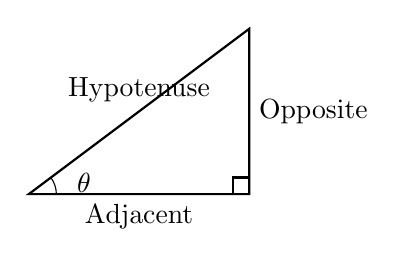
\begin{tikzpicture}[scale=0.7]
        \draw[thick] (0,0) -- (4,0) -- (4,3) -- cycle;
        \draw[thick] (3.7,0) -- (3.7,0.3) -- (4,0.3);
        \node[right] at (4,1.5) {Opposite};
        \node[below] at (2,0) {Adjacent};
        \node[above, sloped] at (2,1.5) {Hypotenuse};
        \draw (0.5,0) arc (0:36.87:0.5);
        \node[right] at (0.7,0.2) {$\theta$};
    \end{tikzpicture}
    \end{center}
\end{frame}

% 3.1 Basic Trigonometric Functions Practice
\begin{frame}{3.1 Practice Problems / 練習題}
    \begin{tcolorbox}[colback=lightgray,colframe=accent,title=Practice]
        \footnotesize
        \begin{enumerate}
            \item Find $\sin 30^\circ$, $\cos 60^\circ$, $\tan 45^\circ$.
            \item In a right triangle, if $\theta = 37^\circ$ and hypotenuse $= 10$, find the length of the side opposite $\theta$.
            \item If $\sin \theta = 0.6$ and $\theta$ is acute, find $\cos \theta$.
            \item Given a right triangle with legs 5 and 12, find all three basic trig ratios for the non-right angles.
        \end{enumerate}
    \end{tcolorbox}
\end{frame}

\begin{frame}{3.1 Solutions / 解答}
    \begin{tcolorbox}[colback=lightgray,colframe=accent,title=Solutions]
        \footnotesize
        \begin{enumerate}
            \item $\sin 30^\circ = 0.5$, $\cos 60^\circ = 0.5$, $\tan 45^\circ = 1$
            \item $\text{Opposite} = 10 \times \sin 37^\circ \approx 6.02$
            \item $\cos \theta = \sqrt{1 - (0.6)^2} = 0.8$
            \item Hypotenuse $= \sqrt{5^2 + 12^2} = 13$; $\sin = 5/13$, $\cos = 12/13$, $\tan = 5/12$
        \end{enumerate}
    \end{tcolorbox}
\end{frame}

% 3.2 Angles in Standard Position
\begin{frame}{3.2 Angles in Standard Position / 標準位置的角}
    \begin{tcolorbox}[colback=lightgray,colframe=primary,title=Key Points]
        \footnotesize
        \begin{itemize}
            \item Angles measured from the positive $x$-axis
            \item Quadrants I-IV
            \item Reference angle: always positive, between terminal arm and $x$-axis
        \end{itemize}
    \end{tcolorbox}
    \vspace{0.5em}
    \begin{center}
    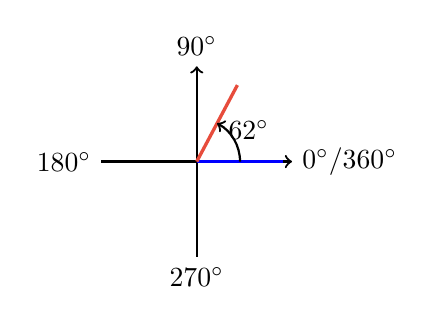
\begin{tikzpicture}[scale=1.1]
        \draw[thick,->] (-1.1,0) -- (1.1,0) node[right] {$0^\circ$/$360^\circ$};
        \draw[thick,->] (0,-1.1) -- (0,1.1) node[above] {$90^\circ$};
        \draw[thick] (-1,0) -- (-1.1,0) node[left] {$180^\circ$};
        \draw[thick] (0,-1) -- (0,-1.1) node[below] {$270^\circ$};
        \draw[very thick,blue] (0,0) -- (1,0);
        \draw[very thick,accent] (0,0) -- ({cos(62)},{sin(62)});
        \draw[->,thick] (0.5,0) arc (0:62:0.5);
        \node at ({0.7*cos(31)},{0.7*sin(31)}) {$62^\circ$};
    \end{tikzpicture}
    \end{center}
\end{frame}

% 3.2 Angles in Standard Position Practice
\begin{frame}{3.2 Practice Problems / 練習題}
    \begin{tcolorbox}[colback=lightgray,colframe=accent,title=Practice]
        \footnotesize
        \begin{enumerate}
            \item Draw $120^\circ$ in standard position and label the reference angle.
            \item What is the reference angle for $210^\circ$?
            \item In which quadrant does $-75^\circ$ lie?
            \item Find the reference angle for $-135^\circ$.
        \end{enumerate}
    \end{tcolorbox}
\end{frame}

\begin{frame}{3.2 Solutions / 解答}
    \begin{tcolorbox}[colback=lightgray,colframe=accent,title=Solutions]
        \footnotesize
        \begin{enumerate}
            \item Reference angle is $180^\circ - 120^\circ = 60^\circ$
            \item $210^\circ$ is in QIII, reference angle $= 210^\circ - 180^\circ = 30^\circ$
            \item $-75^\circ$ is in QIV
            \item $-135^\circ$ is in QIII, reference angle $= 180^\circ - 135^\circ = 45^\circ$
        \end{enumerate}
    \end{tcolorbox}
\end{frame}

% 3.3 Special Triangles
\begin{frame}{3.3 Special Triangles / 特殊三角形}
    \begin{tcolorbox}[colback=lightgray,colframe=primary,title=Key Points]
        \footnotesize
        \begin{itemize}
            \item $30^\circ$-$60^\circ$-$90^\circ$ and $45^\circ$-$45^\circ$-$90^\circ$ triangles
            \item Exact values for $\sin$, $\cos$, $\tan$ of special angles
        \end{itemize}
    \end{tcolorbox}
    \vspace{0.5em}
    \begin{columns}
        \column{0.5\textwidth}
        \centering
        $30^\circ$-$60^\circ$-$90^\circ$
        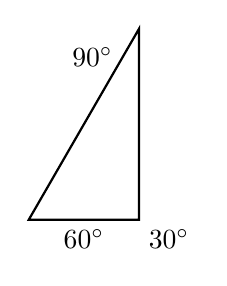
\begin{tikzpicture}[scale=0.7]
            \draw[thick] (0,0) -- (2,0) -- (2,3.464) -- cycle;
            \node[below] at (1,0) {$60^\circ$};
            \node[above left] at (1.7,2.6) {$90^\circ$};
            \node[below right] at (2,0) {$30^\circ$};
        \end{tikzpicture}
        \column{0.5\textwidth}
        \centering
        $45^\circ$-$45^\circ$-$90^\circ$
        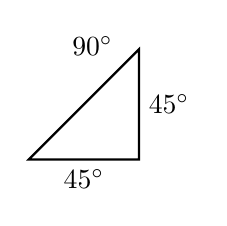
\begin{tikzpicture}[scale=0.7]
            \draw[thick] (0,0) -- (2,0) -- (2,2) -- cycle;
            \node[below] at (1,0) {$45^\circ$};
            \node[right] at (2,1) {$45^\circ$};
            \node[above left] at (1.7,1.7) {$90^\circ$};
        \end{tikzpicture}
    \end{columns}
\end{frame}

% 3.3 Special Triangles Practice
\begin{frame}{3.3 Practice Problems / 練習題}
    \begin{tcolorbox}[colback=lightgray,colframe=accent,title=Practice]
        \footnotesize
        \begin{enumerate}
            \item Find $\sin 60^\circ$ using a special triangle.
            \item Find $\tan 30^\circ$ using a special triangle.
            \item What are the side ratios for a $45^\circ$-$45^\circ$-$90^\circ$ triangle?
            \item Find $\cos 45^\circ$ using a special triangle.
        \end{enumerate}
    \end{tcolorbox}
\end{frame}

\begin{frame}{3.3 Solutions / 解答}
    \begin{tcolorbox}[colback=lightgray,colframe=accent,title=Solutions]
        \footnotesize
        \begin{enumerate}
            \item $\sin 60^\circ = \frac{\sqrt{3}}{2}$
            \item $\tan 30^\circ = \frac{1}{\sqrt{3}} = \frac{\sqrt{3}}{3}$
            \item $1:1:\sqrt{2}$
            \item $\cos 45^\circ = \frac{1}{\sqrt{2}} = \frac{\sqrt{2}}{2}$
        \end{enumerate}
    \end{tcolorbox}
\end{frame}

% 3.4 Solving Angles in All Four Quadrants
\begin{frame}{3.4 Solving Angles in All Four Quadrants / 四象限解角}
    \begin{tcolorbox}[colback=lightgray,colframe=primary,title=Key Points]
        \footnotesize
        \begin{itemize}
            \item ASTC rule: All Students Take Calculus (signs of trig functions in each quadrant)
            \item Reference angle method for finding all solutions
        \end{itemize}
    \end{tcolorbox}
    \vspace{0.5em}
    \begin{center}
    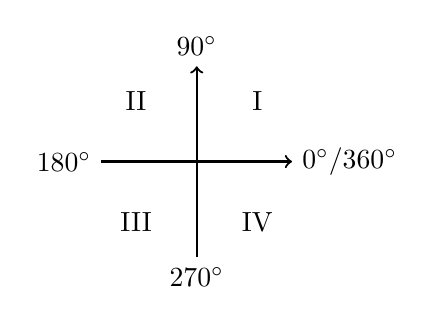
\begin{tikzpicture}[scale=1.1]
        \draw[thick,->] (-1.1,0) -- (1.1,0) node[right] {$0^\circ$/$360^\circ$};
        \draw[thick,->] (0,-1.1) -- (0,1.1) node[above] {$90^\circ$};
        \draw[thick] (-1,0) -- (-1.1,0) node[left] {$180^\circ$};
        \draw[thick] (0,-1) -- (0,-1.1) node[below] {$270^\circ$};
        \node at (0.7,0.7) {I};
        \node at (-0.7,0.7) {II};
        \node at (-0.7,-0.7) {III};
        \node at (0.7,-0.7) {IV};
    \end{tikzpicture}
    \end{center}
\end{frame}

% 3.4 Solving Angles in All Four Quadrants Practice
\begin{frame}{3.4 Practice Problems / 練習題}
    \begin{tcolorbox}[colback=lightgray,colframe=accent,title=Practice]
        \footnotesize
        \begin{enumerate}
            \item Find all angles $0^\circ < \theta < 360^\circ$ where $\sin \theta = 0.5$.
            \item Find all angles $0^\circ < \theta < 360^\circ$ where $\tan \theta = -1$.
            \item In which quadrants is $\cos \theta$ negative?
            \item Find all solutions for $\sin \theta = -\frac{\sqrt{2}}{2}$ in $0^\circ < \theta < 360^\circ$.
        \end{enumerate}
    \end{tcolorbox}
\end{frame}

\begin{frame}{3.4 Solutions / 解答}
    \begin{tcolorbox}[colback=lightgray,colframe=accent,title=Solutions]
        \footnotesize
        \begin{enumerate}
            \item $\theta = 30^\circ, 150^\circ$
            \item $\theta = 135^\circ, 315^\circ$
            \item QII and QIII
            \item $225^\circ, 315^\circ$
        \end{enumerate}
    \end{tcolorbox}
\end{frame}

% 3.5 Sine Law
\begin{frame}{3.5 Sine Law / 正弦定理}
    \begin{tcolorbox}[colback=lightgray,colframe=primary,title=Key Points]
        \footnotesize
        \begin{itemize}
            \item Sine Law: $\frac{a}{\sin A} = \frac{b}{\sin B} = \frac{c}{\sin C}$
            \item Use for non-right triangles when you have an angle and its opposite side
        \end{itemize}
    \end{tcolorbox}
    \vspace{0.5em}
    \begin{center}
    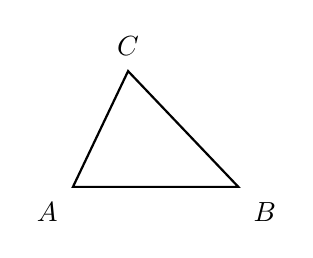
\begin{tikzpicture}[scale=0.7]
        \coordinate (A) at (0,0);
        \coordinate (B) at (3,0);
        \coordinate (C) at (1,2.1);
        \draw[thick] (A) -- (B) -- (C) -- cycle;
        \node[below left=2pt] at (A) {$A$};
        \node[below right=2pt] at (B) {$B$};
        \node[above=2pt] at (C) {$C$};
    \end{tikzpicture}
    \end{center}
\end{frame}

% 3.5 Sine Law Practice
\begin{frame}{3.5 Practice Problems / 練習題}
    \begin{tcolorbox}[colback=lightgray,colframe=accent,title=Practice]
        \footnotesize
        \begin{enumerate}
            \item In $\triangle ABC$, $a=7$, $A=40^\circ$, $B=60^\circ$. Find $b$.
            \item In $\triangle ABC$, $a=10$, $A=30^\circ$, $c=12$, $C=80^\circ$. Find $b$.
            \item In $\triangle ABC$, $a=8$, $A=50^\circ$, $b=10$. Find $B$.
            \item In $\triangle ABC$, $a=9$, $A=35^\circ$, $c=11$. Find $C$.
        \end{enumerate}
    \end{tcolorbox}
\end{frame}

\begin{frame}{3.5 Solutions / 解答}
    \begin{tcolorbox}[colback=lightgray,colframe=accent,title=Solutions]
        \footnotesize
        \begin{enumerate}
            \item $\frac{a}{\sin A} = \frac{b}{\sin B} \Rightarrow b = \frac{7 \sin 60^\circ}{\sin 40^\circ} \approx 9.25$
            \item $\frac{a}{\sin A} = \frac{c}{\sin C} \Rightarrow b = \frac{a \sin B}{\sin A}$, $B = 180^\circ - A - C = 70^\circ$, $b = \frac{10 \sin 70^\circ}{\sin 30^\circ} \approx 18.79$
            \item $\frac{a}{\sin A} = \frac{b}{\sin B} \Rightarrow \sin B = \frac{b \sin A}{a} = \frac{10 \sin 50^\circ}{8} \approx 0.9589$, $B \approx 73.7^\circ$
            \item $\frac{a}{\sin A} = \frac{c}{\sin C} \Rightarrow \sin C = \frac{11 \sin 35^\circ}{9} \approx 0.7005$, $C \approx 44.4^\circ$
        \end{enumerate}
    \end{tcolorbox}
\end{frame}

% 3.6 Ambiguous Case of the Sine Law
\begin{frame}{3.6 Ambiguous Case of the Sine Law / 正弦定理的歧義情形}
    \begin{tcolorbox}[colback=lightgray,colframe=primary,title=Key Points]
        \footnotesize
        \begin{itemize}
            \item SSA case: two sides and a non-included angle
            \item May yield 0, 1, or 2 possible triangles
            \item Check for ambiguous case when using Sine Law
        \end{itemize}
    \end{tcolorbox}
    \vspace{0.5em}
    \begin{center}
    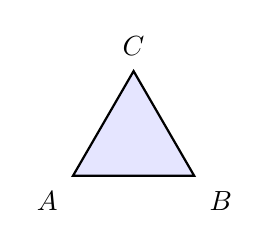
\begin{tikzpicture}[scale=0.7]
        \coordinate (A) at (0,0);
        \coordinate (B) at (2.2,0);
        \coordinate (C) at (1.1,1.9);
        \fill[blue!10] (A) -- (B) -- (C) -- cycle;
        \draw[thick] (A) -- (B) -- (C) -- cycle;
        \node[below left=2pt] at (A) {$A$};
        \node[below right=2pt] at (B) {$B$};
        \node[above=2pt] at (C) {$C$};
    \end{tikzpicture}
    \end{center}
\end{frame}

% 3.6 Ambiguous Case of the Sine Law Practice
\begin{frame}{3.6 Practice Problems / 練習題}
    \begin{tcolorbox}[colback=lightgray,colframe=accent,title=Practice]
        \footnotesize
        \begin{enumerate}
            \item In $\triangle ABC$, $a=8$, $b=10$, $A=30^\circ$. How many possible triangles?
            \item In $\triangle ABC$, $a=7$, $b=12$, $A=40^\circ$. Find all possible values for $B$.
            \item In $\triangle ABC$, $a=9$, $b=8$, $A=50^\circ$. Find all possible values for $B$.
            \item In $\triangle ABC$, $a=6$, $b=5$, $A=25^\circ$. How many possible triangles?
        \end{enumerate}
    \end{tcolorbox}
\end{frame}

\begin{frame}{3.6 Solutions / 解答}
    \begin{tcolorbox}[colback=lightgray,colframe=accent,title=Solutions]
        \footnotesize
        \begin{enumerate}
            \item $a < b$, $a > b \sin A$ so 2 triangles possible
            \item $\sin B = \frac{12 \sin 40^\circ}{7} \approx 1.099$ (no triangle)
            \item $\sin B = \frac{8 \sin 50^\circ}{9} \approx 0.682$, $B_1 = 43^\circ$, $B_2 = 137^\circ$
            \item $\sin B = \frac{5 \sin 25^\circ}{6} \approx 0.352$, $B_1 = 20.6^\circ$, $B_2 = 159.4^\circ$
        \end{enumerate}
    \end{tcolorbox}
\end{frame}

% 3.7 Cosine Law
\begin{frame}{3.7 Cosine Law / 餘弦定理}
    \begin{tcolorbox}[colback=lightgray,colframe=primary,title=Key Points]
        \footnotesize
        \begin{itemize}
            \item Cosine Law: $a^2 = b^2 + c^2 - 2bc\cos A$ (and cyclic)
            \item Use for non-right triangles with SAS or SSS
        \end{itemize}
    \end{tcolorbox}
    \vspace{0.5em}
    \begin{center}
    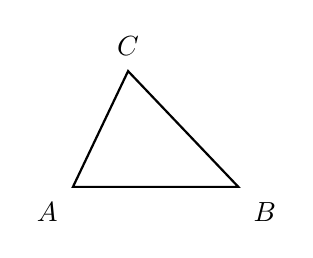
\begin{tikzpicture}[scale=0.7]
        \coordinate (A) at (0,0);
        \coordinate (B) at (3,0);
        \coordinate (C) at (1,2.1);
        \draw[thick] (A) -- (B) -- (C) -- cycle;
        \node[below left=2pt] at (A) {$A$};
        \node[below right=2pt] at (B) {$B$};
        \node[above=2pt] at (C) {$C$};
    \end{tikzpicture}
    \end{center}
\end{frame}

% 3.7 Cosine Law Practice
\begin{frame}{3.7 Practice Problems / 練習題}
    \begin{tcolorbox}[colback=lightgray,colframe=accent,title=Practice]
        \footnotesize
        \begin{enumerate}
            \item In $\triangle ABC$, $a=7$, $b=8$, $C=60^\circ$. Find $c$.
            \item In $\triangle ABC$, $a=10$, $b=12$, $c=15$. Find $A$.
            \item In $\triangle ABC$, $a=9$, $b=11$, $C=45^\circ$. Find $c$.
            \item In $\triangle ABC$, $a=5$, $b=7$, $c=8$. Find $B$.
        \end{enumerate}
    \end{tcolorbox}
\end{frame}

\begin{frame}{3.7 Solutions / 解答}
    \begin{tcolorbox}[colback=lightgray,colframe=accent,title=Solutions]
        \footnotesize
        \begin{enumerate}
            \item $c^2 = 7^2 + 8^2 - 2 \times 7 \times 8 \cos 60^\circ = 49 + 64 - 112 \times 0.5 = 113 - 56 = 57$, $c = \sqrt{57} \approx 7.55$
            \item $A = \cos^{-1}\left(\frac{10^2 + 12^2 - 15^2}{2 \times 10 \times 12}\right) = \cos^{-1}\left(\frac{100+144-225}{240}\right) = \cos^{-1}(-0.3375) \approx 110.7^\circ$
            \item $c^2 = 9^2 + 11^2 - 2 \times 9 \times 11 \cos 45^\circ = 81 + 121 - 198 \times 0.7071 = 202 - 140 = 62$, $c = \sqrt{62} \approx 7.87$
            \item $B = \cos^{-1}\left(\frac{5^2 + 8^2 - 7^2}{2 \times 5 \times 8}\right) = \cos^{-1}\left(\frac{25+64-49}{80}\right) = \cos^{-1}(0.5) = 60^\circ$
        \end{enumerate}
    \end{tcolorbox}
\end{frame}

% Final Review Questions
\begin{frame}{Final Review Questions / 綜合練習}
    \begin{tcolorbox}[colback=lightgray,colframe=primary,title=Comprehensive Review]
        \footnotesize
        \begin{enumerate}
            \item Find $\sin 45^\circ$, $\cos 60^\circ$, $\tan 30^\circ$
            \item Draw an angle of $120^\circ$ in standard position and label the reference angle
            \item Solve $\triangle ABC$ given $A=40^\circ$, $a=7$, $b=10$
            \item Use the Sine Law to find a missing side
            \item Use the Cosine Law to find a missing angle
            \item Explain the ambiguous case for Sine Law
        \end{enumerate}
    \end{tcolorbox}
\end{frame}

\end{document} 